 \documentclass[a4paper, 14pt, oneside]{extbook}
\usepackage[T1]{fontenc}
\usepackage[utf8x]{inputenc}
\usepackage[italian]{babel}
\usepackage[hmargin=2cm, top=2.5cm, bottom=3.5cm]{geometry}
\usepackage{courier}
\usepackage{hyperref}
\usepackage{url}  % Per gestire gli URL nella bibliografia

% Grafica
\usepackage[table]{xcolor}
\usepackage{tabularx}
\usepackage{graphicx,pstricks}
\usepackage{graphics}
\usepackage{float}
\usepackage{pdflscape}
\graphicspath{{img/}}

% Package usati per il frontespizio
\usepackage{tikz}
\usepackage{pgf-pie}
\usepackage{pgfplots}
\pgfplotsset{width=7cm,compat=1.8}
\usetikzlibrary{patterns}

%Chapter
\usepackage{titlesec}
\titlespacing*{\chapter}{0pt}{-\baselineskip}{20pt}
\titleformat{\chapter}[display]
  {\normalfont\huge\bfseries}{\chaptertitlename\ \thechapter}{20pt}{\huge}[\vspace{4pt}\color{darkgray!90}\titlerule]

%Formatting
\usepackage{changepage}
\newenvironment{mychapter}[1]{\chapter{#1}\begin{adjustwidth}{1cm}{0cm}}{\end{adjustwidth}}
\newenvironment{mychapterstar}[1]{\chapter*{#1}\begin{adjustwidth}{1cm}{0cm}}{\end{adjustwidth}}
\newenvironment{mysection}[1]{\begin{adjustwidth}{-1cm}{0cm}\section{#1}\end{adjustwidth}}{}
\newenvironment{mysubsection}[1]{\begin{adjustwidth}{-1cm}{0cm}\subsection{#1}\end{adjustwidth}}{}

%Algorithm
\usepackage{algorithm}
\usepackage[noend]{algpseudocode}

%Code snippets
\usepackage{listings}
\lstdefinestyle{mycode}{
    backgroundcolor=\color{gray!10},
    basicstyle=\ttfamily\small,
    breaklines=true,
    frame=single,
    rulecolor=\color{gray!40},
    numbers=left,
    numbersep=5pt,
    numberstyle=\tiny\color{gray},
    showstringspaces=false,
    tabsize=2,
    captionpos=b,
}
\lstset{style=mycode}

%Hyphenation
\tolerance=1
\emergencystretch=\maxdimen
\hyphenpenalty=10000
\hbadness=10000

%Header
\usepackage{fancyhdr}
\makeatletter
\newcommand{\mytitle}{\@title}
\makeatother
\setlength{\headheight}{52pt}

\fancypagestyle{plain}{%
  \fancyhf{}%
  \fancyhead[L]{
\includegraphics[scale=0.35]{img/logo_copertina_1.png}}
  \fancyhead[R]{\begin{minipage}[b]{.66\textwidth}\hfill\mytitle\end{minipage}}
  \fancyfoot[C]{\thepage}
}
\AtBeginDocument{\addtocontents{toc}{\protect\thispagestyle{empty}}} 

%Other
\usepackage{comment}
\usepackage{amsmath}
\usepackage{fix-cm}

%bibliografia
\usepackage{biblatex}
\addbibresource{bibliography.bib}



%=======================================================================================================================================

\title{Scalamarket: Using API, Kubernetes and AWS for developing a Microservice-based E-Commerce Platform}

\begin{document}

\begin{titlepage}
\thispagestyle{empty}
\raggedright 
% Define \mysubtitle if not provided to avoid Undefined control sequence
\providecommand{\mysubtitle}{}

\begin{tikzpicture}
\node[anchor=south west] at (5,0) {
\includegraphics[scale=0.75]{img/logo_copertina_1}};
\node[anchor=south west] at (0,0.9) {
\includegraphics{img/logo_copertina_2}};
\node[anchor=south west] at (0,-1) {\textsf{\fontsize{15}{60}\selectfont \textbf{Cloud Platform And Infrastructure as Code}}}; %<----- MODIFY HERE <-----
\end{tikzpicture}

\vfill

\vspace{3cm}

{\bfseries\itshape\LARGE \mytitle \par} % CHANGE THE TITLE ON "MAIN.TEX", NOT HERE
\vspace{0.5cm}
{\textbf{\textit{\Large \mysubtitle}}}
\vspace{1cm}
\vfill

\begin{table}[h]

\textbf{De Lucia Simone M63001720}\\ 
\end{table}

\end{titlepage}
\pagestyle{empty}
\frontmatter

%\newpage
%\cleardoublepage
%\vspace*{\stretch{1}}
%\begin{flushright}
%\itshape Una dedica\\


%\end{flushright}
\vspace{\stretch{2}}
\cleardoublepage

\tableofcontents

\mainmatter
\pagestyle{plain}

\begin{mychapter}{Presentazione del Progetto}

\begin{mysection}{Descrizione Generale}
Scalamarket è una moderna piattaforma e-commerce basata su un'architettura a microservizi, progettata per garantire elevata scalabilità, affidabilità e flessibilità. Il sistema gestisce l'intero ciclo di vita dell'acquisto online: dalla registrazione degli utenti, alla consultazione del catalogo, fino all'elaborazione degli ordini e alla gestione logistica delle spedizioni. L'intera infrastruttura è stata ideata per essere distribuita in modo efficiente tramite Kubernetes ed eventualmente ospitata in ambiente cloud AWS, fornendo un backend solido, scalabile e supportato da API RESTful. 


\begin{figure}[h]
    \centering
    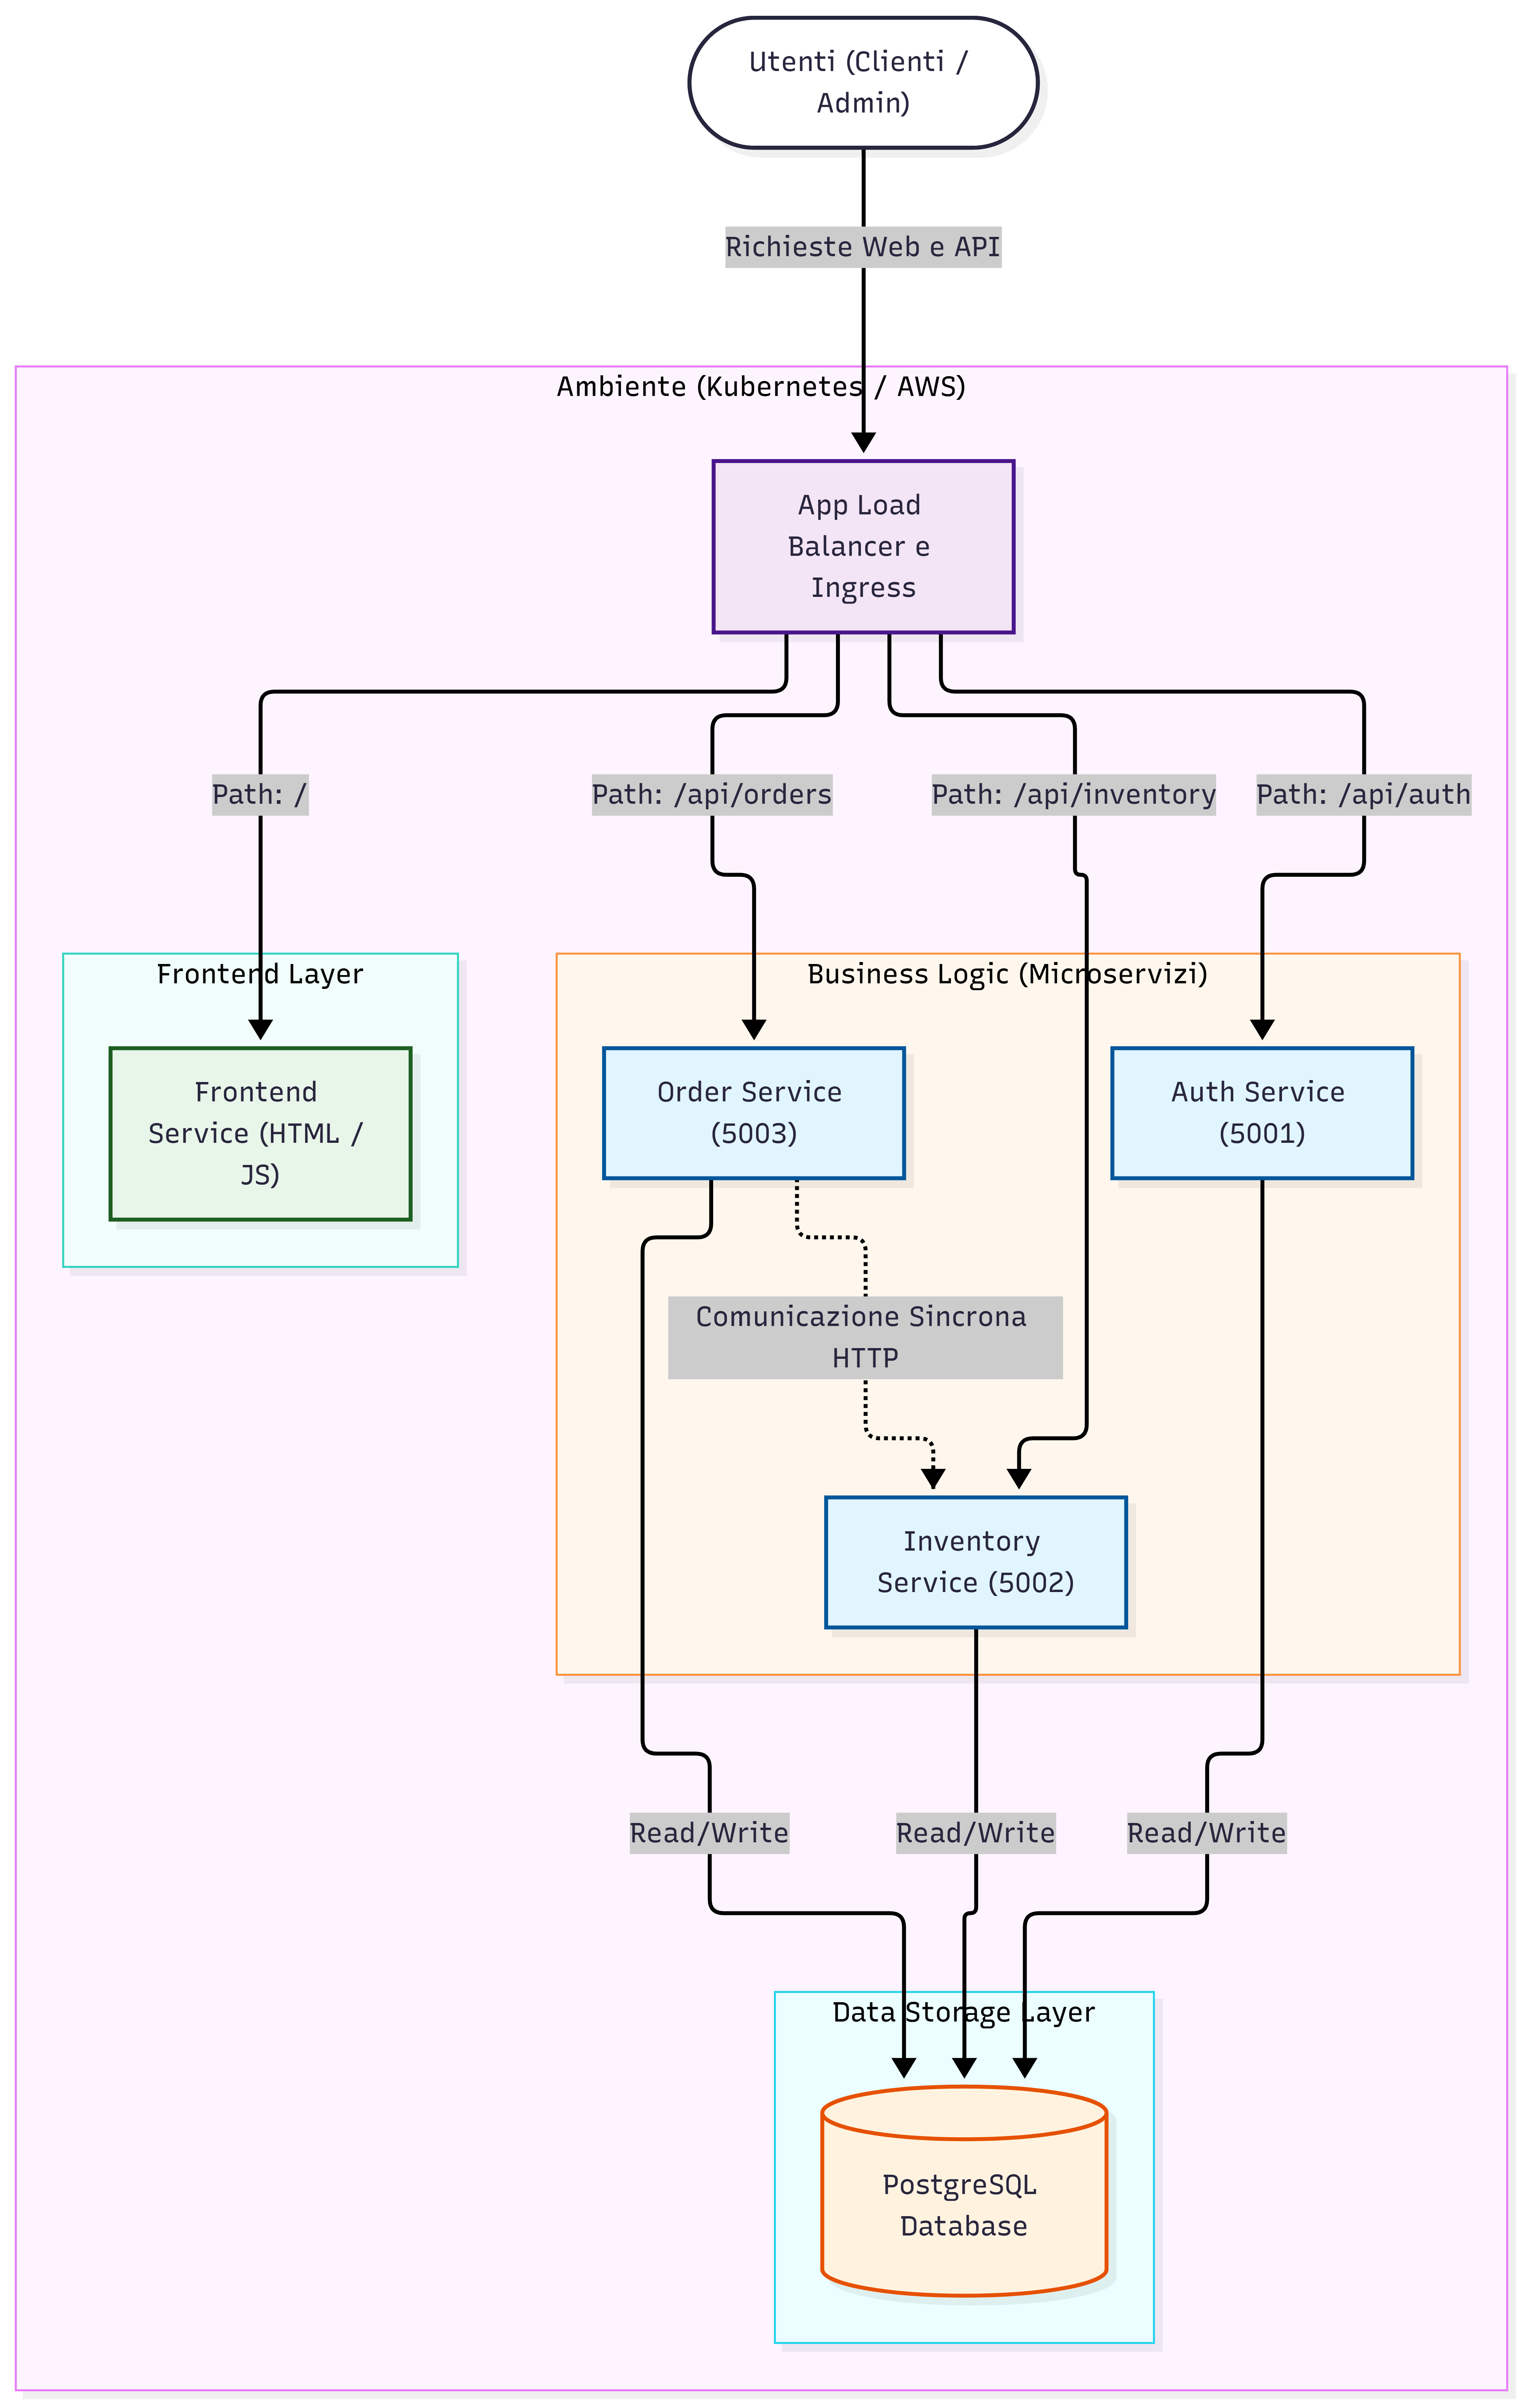
\includegraphics[width=\textwidth,height=0.45\textheight,keepaspectratio]{img/ComponentDiagram.png}
    \caption{Diagramma dei Componenti UML}
    \label{fig:component_diagram}
\end{figure}
\end{mysection}

\begin{mysection}{Requisiti dell'Applicativo}
L'applicativo è stato sviluppato per soddisfare i seguenti requisiti architetturali, funzionali e di business 

\begin{itemize}
    \item \textbf{Autenticazione e Autorizzazione (Auth Service):} Il sistema deve permettere la registrazione e il login sicuri sia per i clienti (Client) che per gli amministratori (Admin). L'amministratore deve avere i privilegi per gestire le utenze.
    \item \textbf{Gestione Inventario (Inventory Service):} Il sistema deve gestire un catalogo dinamico di articoli, tenendo traccia delle quantità ripartite in molteplici filiali. Deve inoltre impedire la creazione di ordini per articoli non disponibili.
    \item \textbf{Gestione Ordini e Logistica (Order Service):} L'applicativo deve processare il carrello dell'utente, allocando in tempo reale i prodotti necessari e scalandoli in modo intelligente dalle filiali che ne hanno disponibilità. Deve inoltre tracciare l'occupazione dei mezzi logistici, gestendo i furgoni in uso e quelli a disposizione.
    \item \textbf{Architettura a Microservizi e Dati Isolati:} Per massimizzare la modularità, ogni servizio deve possedere una propria logica di business e interfacciarsi con il proprio database PostgreSQL indipendente, disaccoppiando così i domini applicativi.
\end{itemize}

È importante specificare che l'applicativo è da considerarsi un Prototipo (Proof of Concept) atto a dimostrare le dinamiche di scalabilità, distribuzione e interazione tra microservizi, e non è pensato per un utilizzo commerciale in produzione. Alcune interfacce, così come la maggior parte delle funzionalità di sicurezza sono da considerarsi basilari

\begin{figure}[h]
    \centering
    \includegraphics[width=\textwidth,height=0.45\textheight,keepaspectratio]{img/SequenceDiagram.png}
    \caption{Diagramma di Sequenza}
    \label{fig:sequence_diagram}
\end{figure}

\end{mysection}

\begin{mysection}{Il Sito Web}
Per l'implementazione di Scalamarket si è scelto un framework Flask. Il lato client e il pannello di gestione amministrativa sono stati realizzati mediante un'interfaccia web responsive integrata con il backend. L'applicazione espone e gestisce tutti gli endpoint necessari, mentre la UI comunica costantemente con questi servizi tramite chiamate asincrone.

Il sito implementa tre diverse interfacce: \textbf{Cliente}, \textbf{Gestore Filiale} ed \textbf{Amministratore Globale}.

\begin{itemize}
    \item \textbf{Interfaccia Cliente:} L'utente può scorrere l'intero catalogo, visualizzare i prezzi e le disponibilità massime, aggiungere elementi al carrello e, una volta inviato l'ordine, monitorarne lo stato e i dettagli dei prodotti tramite un'apposita cronologia.
    \item \textbf{Interfaccia Amministratore Globale:} L'admin ha accesso a una dashboard completa che gli permette di visualizzare l'inventario globale (con possibilità di ricerca rapida), controllare in tempo reale lo stato logistico totale, visionare ed eliminare lo storico ordini globale e monitorare/eliminare gli account utenti.
    \item \textbf{Interfaccia Gestore Filiale:} Il gestore ha una visione limitata esclusivamente alle giacenze e ai veicoli della propria sede, con i poteri esclusivi di poter aggiungere o rimuovere articoli dal catalogo, e aggiornare le scorte e i mezzi assegnati alla filiale.
\end{itemize}

\textit{Nota: per un'analisi dettagliata e visiva di come è strutturata l'interfaccia utente (UI) nelle sue varie schermate, si rimanda al quinto capitolo, "Interfaccia Utente", del documento.}

\begin{figure}[h]
    \centering
    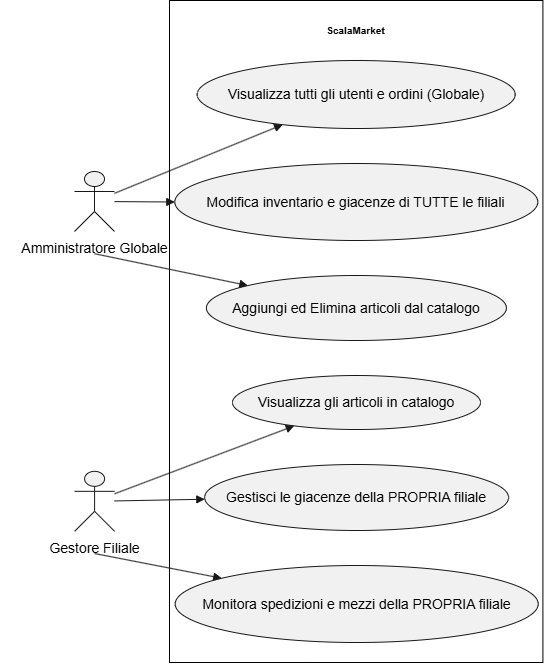
\includegraphics[width=\textwidth,height=0.45\textheight,keepaspectratio]{img/UseCaseDiagram.png}
    \caption{Diagramma dei Casi d'Uso}
    \label{fig:use_case_diagram}
\end{figure}

\end{mysection}

\end{mychapter}

\begin{mychapter}{Orchestrazione Kubernetes}

\begin{mysection}{Infrastruttura del Cluster}
L'infrastruttura Kubernetes poggia su componenti isolati al fine di scalare singolarmente in base alle esigenze e prevenire disservizi totali (\textit{Single Point of Failure}). 

I componenti base dell'applicativo sono i seguenti:
\begin{itemize}
    \item \textbf{frontend} (nginx): Gestisce la GUI per clienti e amministratori, esposto sulla porta 8080.
    \item \textbf{auth-service} (Flask): Gestisce autenticazione, registrazione e ruoli.
    \item \textbf{inventory-service} (Flask): Gestisce il catalogo, articoli e giacenze.
    \item \textbf{order-service} (Flask): Gestisce gli ordini, lo storico e la logistica.
    \item \textbf{postgres}: Database centrale con storage persistente garantito da un \texttt{PersistentVolume} (PV) e un \texttt{PersistentVolumeClaim} (PVC), logicamente frammentato in 3 database separati.
\end{itemize}

\subsubsection*{Ridondanza e Scalabilità}
I servizi stateless (Frontend e Logica di Business) sono stati configurati con repliche multiple, distribuite automaticamente dal \texttt{Service} \texttt{ClusterIP} che funge da load-balancer interno:
\begin{itemize}
    \item \textbf{Frontend (nginx):} 2 repliche per garantire alta disponibilità durante aggiornamenti o guasti di un Pod.
    \item \textbf{Logica di Business (auth, inventory, order):} 3 repliche ciascuno, in quanto soggetti a maggior stress e richieste concorrenti (es. elaborazione parallela ordini o scritture simultanee inventario).
    \item \textbf{Database (postgres):} Rimane a 1 replica. In ambiente nativo relazionale, la coerenza dei dati orizzontale richiede approcci dedicati; mantenere 1 replica ne previene il partizionamento anomalo.
\end{itemize}

Tutti i container Flask sono inoltre dotati di \texttt{resources} (requests e limits) per evitare che un consumo anomalo da parte di un Pod degradi le prestazioni degli altri (\textit{noisy neighbor}).

\subsubsection*{Kubernetes Ingress Controller}
L'accesso esterno e il routing dei servizi avvengono tramite un \textbf{Kubernetes Ingress Controller} (basato su NGINX) che agisce da \textit{reverse proxy} HTTP a livello di cluster. Attraverso un unico indirizzo esposto al pubblico, elimina la necessità di port-forward multipli. Le rotte principali implementate sono:
\begin{itemize}
    \item \texttt{/} $\rightarrow$ \texttt{frontend-service:8080}
    \item \texttt{/api/auth/} $\rightarrow$ \texttt{auth-service:5001}
    \item \texttt{/api/inventory/} $\rightarrow$ \texttt{inventory-service:5002}
    \item \texttt{/api/orders/} $\rightarrow$ \texttt{order-service:5003}
\end{itemize}

\textit{Nota: Si rimanda al quarto capitolo per un analisi più dettagliata delle rotte implementate e quali richieste vengono gestite da ciascuna di esse.}

\subsubsection*{Analisi dei Manifest Kubernetes}
L'architettura descritta è governata da una serie di manifest Kubernetes (file YAML) che dichiarano in maniera esplicita lo stato desiderato dell'infrastruttura.

\begin{itemize}
    \item \textbf{Ingress Locale (\texttt{ingress-local.yaml}):} Definisce le regole di instradamento specificando la \textit{ingressClassName} \texttt{nginx}. La risorsa si suddivide in blocchi \texttt{rules} che incanalano le chiamate ai backend giusti.
    \item \textbf{Deployment di un Microservizio (es. \texttt{order-deployment.yaml}):} Illustra le \textit{best-practice} del deployment stateless in Kubernetes. Specifica \texttt{replicas: 3}, \texttt{imagePullPolicy} e l'iniezione delle \texttt{env} necessarie (come la stringa di connessione DB). Impone infine limiti rigidi sulle \texttt{resources.requests} e \texttt{resources.limits} di CPU/RAM.
    \item \textbf{Deployment del Database (\texttt{postgres-deployment.yaml}):} A differenza dei precedenti, usa i \textit{Volumes}. Integra \texttt{volumeMounts} per i dati nel path \texttt{/var/lib/postgresql/data} collegati a un PVC. Inietta inoltre un \texttt{ConfigMap} nel path \texttt{/docker-entrypoint-initdb.d} per creare i database automaticamente all'avvio.
\end{itemize}

Di seguito viene riportato l'output dell'ambiente locale in esecuzione, che conferma lo stato \texttt{Running} di tutti i pod e la corretta visualizzazione della piattaforma dal browser locale.
\end{mysection}

\begin{figure}[H]
    \centering
    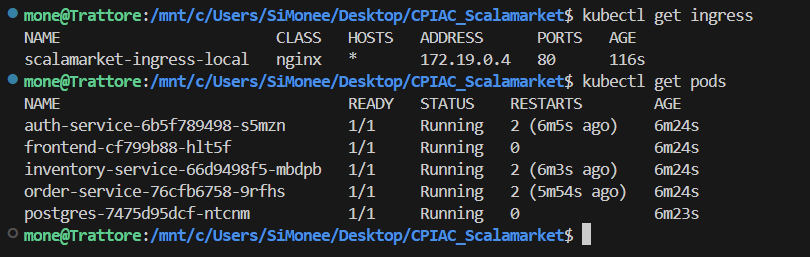
\includegraphics[width=\textwidth]{img/kubectl_local.png}
    \caption{Output del comando \texttt{kubectl get pods} nell'ambiente locale}
    \label{fig:kubectl_local}
\end{figure}

\begin{figure}[H]
    \centering
    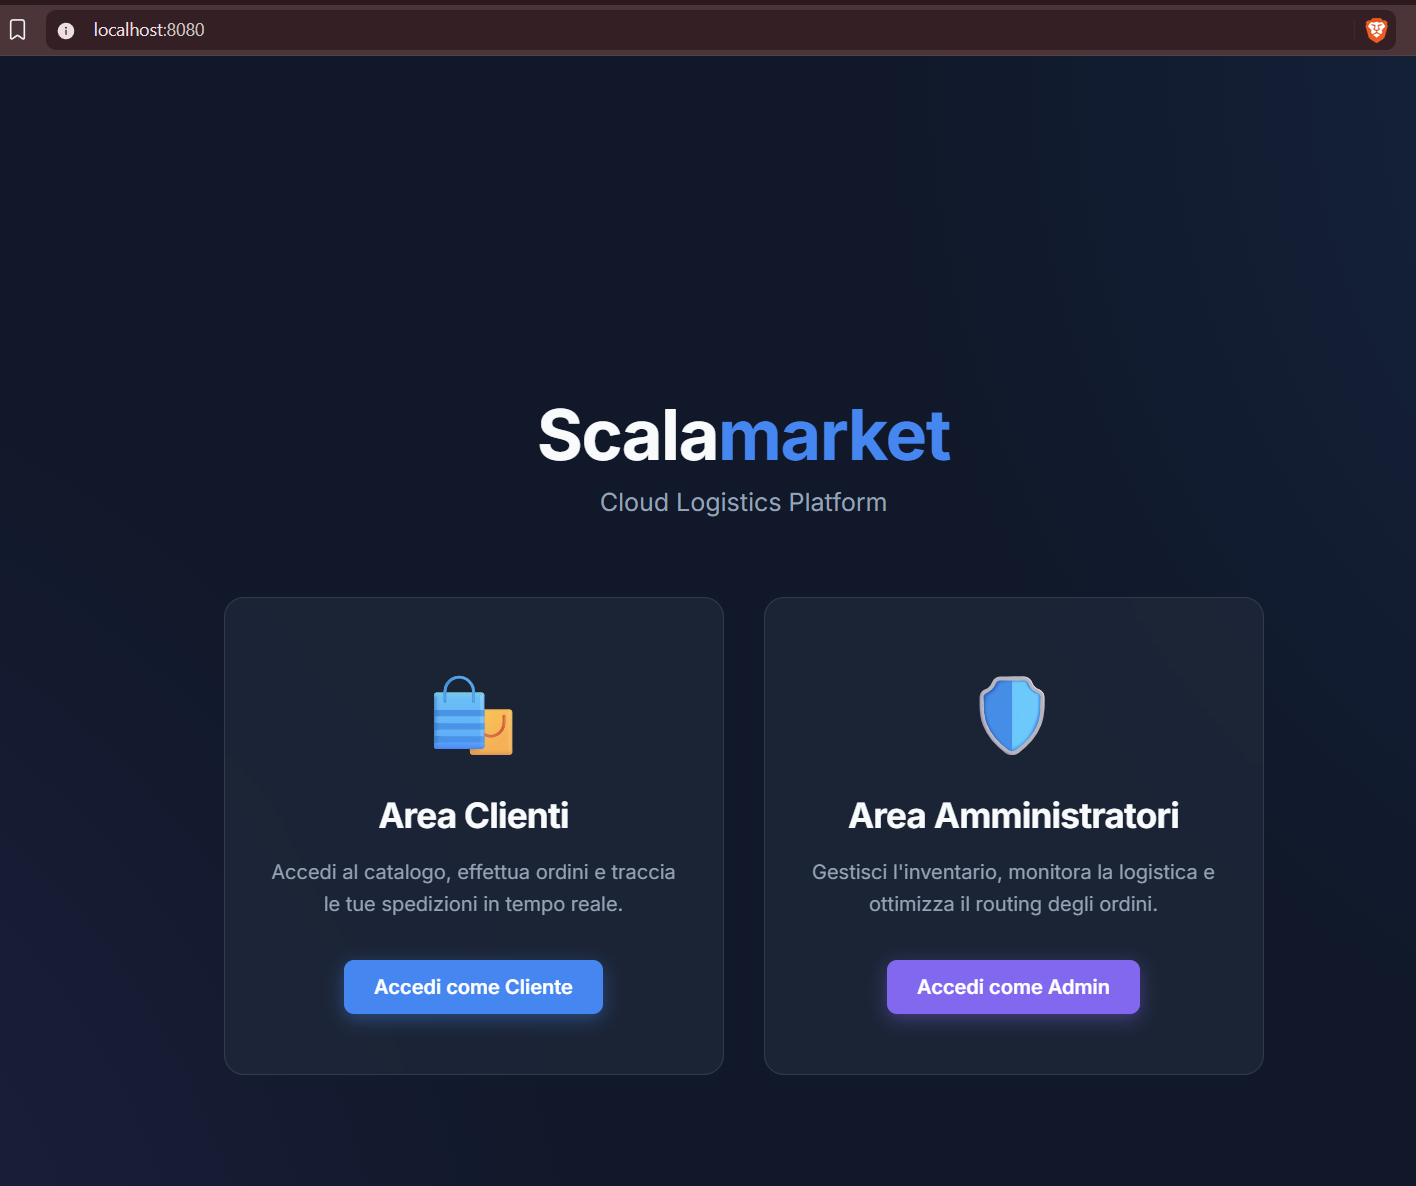
\includegraphics[width=\textwidth]{img/local_deployment.png}
    \caption{Piattaforma correttamente avviata ed esposta tramite localhost}
    \label{fig:local_deployment}
\end{figure}




\end{mychapter}


\begin{mychapter}{Deployment in AWS}

\begin{mysection}{Deployment tramite Infrastructure-as-Code (Terraform)}
Al fine di automatizzare e rendere riproducibile l'infrastruttura Cloud, è stato creato uno script Terraform per effettuare il provisioning delle risorse su Amazon Web Services (AWS).
Questa metodologia, nota come \textit{Infrastructure-as-Code} (IaC), garantisce che la configurazione del cloud sia scritta in file dichiarativi, riducendo l'errore umano.

I file Terraform implementati (\texttt{main.tf}, \texttt{variables.tf}, \texttt{outputs.tf}) descrivono la seguente architettura:
\begin{itemize}
    \item \textbf{VPC e Subnet:} Creazione di una Virtual Private Cloud (VPC) con subnet pubbliche per bilanciatori e risorse accessibili, e subnet private per i nodi Kubernetes.
    \item \textbf{Internet Gateway e Route Tables:} Per consentire il routing verso l'esterno.
    \item \textbf{Security Group:} Regole firewall stateful per aprire le porte in ingresso al traffico HTTP/HTTPS e porte interne per la comunicazione intra-nodo.
    \item \textbf{Application Load Balancer (ALB):} Per distribuire il traffico degli utenti verso i worker node.
    \item \textbf{Istanze EC2:} Lancio di due macchine virtuali distinte (\texttt{t3.medium}) basate su Amazon Machine Image (AMI) Ubuntu: una dedicata alle applicazioni clienti (nella Subnet 1) e una alle applicazioni admin (nella Subnet 2). Lo script \texttt{user\_data.sh} automatizza l'installazione di Docker e delle componenti di Kubernetes (K3s) all'avvio su entrambe.
    \item \textbf{AWS Budgets:} Per evitare costi imprevisti, è configurato un \textit{Monthly Budget} con limite di spesa pari a 100 USD mensili, che invia alert via email se i costi superano la soglia dell'80\%. L'utilizzo di un'architettura essenziale a due nodi garantisce resilienza pur contenendo i costi rispetto a un classico cluster multi-nodo pesante.
\end{itemize}

\begin{figure}[H]
    \centering
    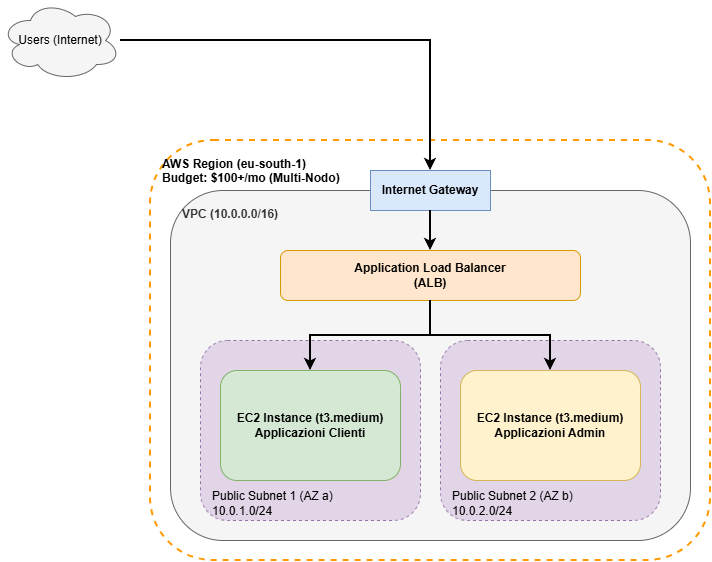
\includegraphics[width=0.9\textwidth]{img/AWSArchitecture.png}
    \caption{Schema Architetturale AWS Multi-Nodo (VPC, Subnet, EC2, ALB)}
    \label{fig:aws_arch}
\end{figure}

\textbf{Load Balancing e Path-Based Routing:}\\
Al fine di separare le competenze mantenendo un singolo punto d'accesso, l'Application Load Balancer (ALB) è stato configurato per effettuare un \textit{Path-Based Routing}. Il traffico in entrata viene analizzato dall'ALB: le richieste dirette ai path \texttt{/admin*} e \texttt{/inventory*} vengono inoltrate automaticamente al \textit{Target Group} del nodo Admin (situato nella Subnet 2), mentre tutte le restanti richieste (di default) sono servite dal \textit{Target Group} del nodo Clienti (nella Subnet 1).

\textbf{Nota sulla configurazione delle credenziali IAM per Terraform:}\\
Per consentire a Terraform di effettuare il provisioning delle risorse su AWS, è necessario configurare correttamente un utente programmatico tramite IAM (Identity and Access Management). Seguendo le best practice illustrate nei tutorial di riferimento (come l'aggiunta dell'utente a un Gruppo IAM specifico), si consiglia di applicare al gruppo la policy predefinita \texttt{AdministratorAccess}. 
Considerando che lo script Terraform necessita di orchestrare contemporaneamente VPC, Security Group, Istanze EC2, Application Load Balancer e impostazioni di Billing (per l'allarme budget), l'accesso amministratore garantisce un'esecuzione senza blocchi o errori di permessi per scopi didattici e di test. In scenari di produzione reali, tuttavia, andrebbe rigorosamente applicato il principio del privilegio minimo (Least Privilege), assemblando policy granulari (ad es. \texttt{AmazonEC2FullAccess}, \texttt{AmazonVPCFullAccess}, ecc.).

\textbf{Selezione dello Use Case per l'Access Key:}\\
Durante la procedura guidata di generazione della coppia di chiavi di accesso (\textit{Access Key} e \textit{Secret Access Key}) nella AWS Console, viene richiesto di specificare l'ambito di utilizzo (\textit{Use case}):
\begin{itemize}
    \item L'opzione da selezionare è \textbf{Command Line Interface (CLI)}. Terraform, infatti, opera interfacciandosi con le API di AWS esattamente come un tool a riga di comando locale (o caricando le credenziali tramite l'AWS CLI configurata con \texttt{aws configure}, oppure leggendo i file \texttt{.aws/credentials} o variabili d'ambiente).
    \item Spuntando la casella di conferma relativa alle raccomandazioni di sicurezza AWS ("I understand the above recommendation and want to proceed..."), è possibile procedere con la generazione e il download del file \texttt{.csv} contenente le chiavi.
\end{itemize}

I passi per eseguire lo script sono i seguenti:
\begin{enumerate}
    \item \textbf{Configurazione Credenziali:} Eseguire \texttt{aws configure} per configurare la CLI con le \textit{Access Keys} ottenute.
    \begin{figure}[H]
        \centering
        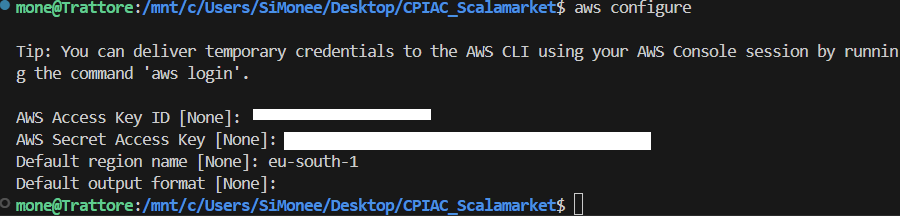
\includegraphics[width=0.7\textwidth]{img/awsConfigure.png}
        \caption{Configurazione tramite AWS CLI}
        \label{fig:aws_configure}
    \end{figure}
    \item \textbf{Inizializzazione:} Eseguire \texttt{terraform init}.
    \begin{figure}[H]
        \centering
        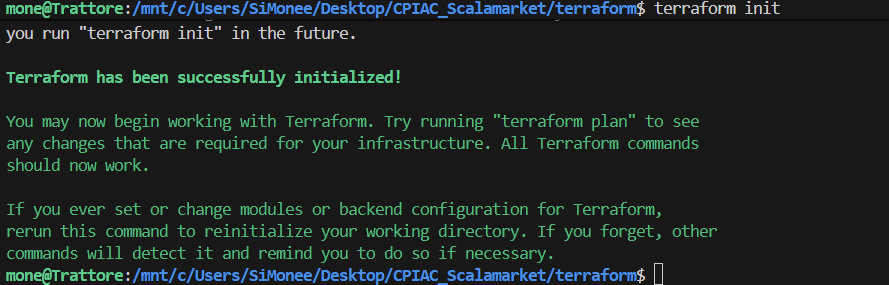
\includegraphics[width=0.7\textwidth]{img/terraformInit.png}
        \caption{Inizializzazione di Terraform}
        \label{fig:terraform_init}
    \end{figure}
    \item \textbf{Verifica e Applicazione:} Eseguire \texttt{terraform plan} e infine \texttt{terraform apply}.
    \begin{figure}[H]
        \centering
        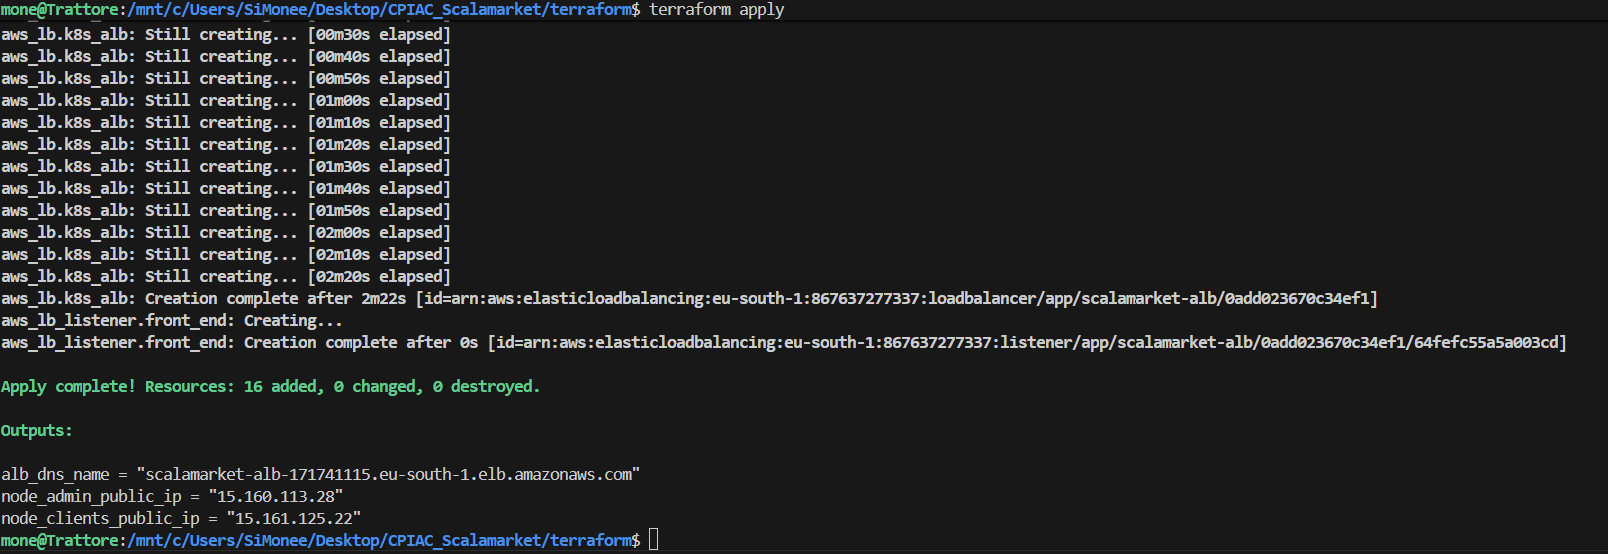
\includegraphics[width=0.7\textwidth]{img/TerraformApply.png}
        \caption{Output del comando Terraform Apply}
        \label{fig:terraform_apply}
    \end{figure}
\end{enumerate}

\textbf{Accesso Remoto e Deploy Applicativo:}\\
Al termine dell'esecuzione di Terraform, verranno stampati a video il DNS name dell'ALB e gli IP Pubblici delle due istanze EC2. 
L'infrastruttura a questo punto è in esecuzione, ma le applicazioni devono ancora essere deployate. I passaggi sono:
\begin{itemize}
    \item \textbf{Accesso SSH:} Collegarsi in SSH alle macchine tramite la chiave definita (es. \texttt{scalamarket-key}).
    \item \textbf{Clone Selettivo (Sparse-Checkout):} Per evitare di scaricare file inutili ai fini del deploy (come questa documentazione o i file Terraform), utilizzare i seguenti comandi su entrambi i nodi:
    \begin{verbatim}
    git clone --no-checkout <TUO_URL_GIT>
    cd CPIAC_Scalamarket
    git sparse-checkout init --cone
    git sparse-checkout set frontend init-scripts microservices k8s
    git checkout main
    \end{verbatim}
    \item \textbf{Deploy K8s - Nodo Clienti:} (Assicurarsi di essere nella cartella \texttt{CPIAC\_Scalamarket})
    \begin{verbatim}
    sudo docker build -t cpiac_frontend:v5 -f frontend/Dockerfile frontend/
    sudo docker build -t cpiac_auth:v5    -f microservices/auth_service/Dockerfile .
    sudo docker build -t cpiac_order:v5   -f microservices/order_service/Dockerfile .

    sudo kubectl apply -f k8s/postgres-pv-pvc.yaml
    sudo kubectl apply -f k8s/postgres-configmap.yaml
    sudo kubectl apply -f k8s/postgres-deployment.yaml
    sudo kubectl apply -f k8s/postgres-service.yaml

    sudo kubectl apply -f k8s/frontend-deployment.yaml
    sudo kubectl apply -f k8s/frontend-service.yaml
    sudo kubectl apply -f k8s/auth-deployment.yaml
    sudo kubectl apply -f k8s/auth-service.yaml
    sudo kubectl apply -f k8s/order-deployment.yaml
    sudo kubectl apply -f k8s/order-service.yaml
    sudo kubectl apply -f k8s/ingress.yaml
    \end{verbatim}
    
    \item \textbf{Deploy K8s - Nodo Admin:}
    \begin{verbatim}
    sudo docker build -t cpiac_inventory:v5 -f microservices/inventory_service/Dockerfile .

    sudo kubectl apply -f k8s/postgres-pv-pvc.yaml
    sudo kubectl apply -f k8s/postgres-configmap.yaml
    sudo kubectl apply -f k8s/postgres-deployment.yaml
    sudo kubectl apply -f k8s/postgres-service.yaml

    sudo kubectl apply -f k8s/inventory-deployment.yaml
    sudo kubectl apply -f k8s/inventory-service.yaml
    sudo kubectl apply -f k8s/ingress.yaml
    \end{verbatim}
    \item \textbf{Navigazione:} Accedere dal browser non tramite gli IP delle macchine, ma tramite l'URL fornito dall'Application Load Balancer (DNS Name). L'ALB smisterà automaticamente il traffico basandosi sul \textit{path} dell'URL.
\end{itemize}
\end{mysection}

\begin{mysection}{Deployment tramite AWS Management Console (GUI)}
In alternativa, è possibile creare manualmente la stessa infrastruttura descritta al paragrafo precedente direttamente tramite il portale web di AWS. Questo approccio è utile a scopo esplorativo e didattico.

Di seguito i passaggi principali:
\begin{enumerate}
    \item \textbf{Creazione VPC:} Dalla sezione VPC, utilizzare il wizard "VPC and more" per creare la rete, specificando il CIDR block e includendo un Internet Gateway.
    \item \textbf{Configurazione Subnet e Route Table:} Separare logicamente le reti pubbliche e private.
    \item \textbf{Lancio Istanze EC2:} Dalla dashboard EC2, cliccare su "Launch Instance". Selezionare un'AMI Ubuntu, scegliere una classe di istanza (es. \texttt{t3.medium}), associare una coppia di chiavi SSH e collocare l'istanza nella subnet corretta associandole un Security Group che apra la porta 22 (SSH) e la 80 (HTTP).
    \item \textbf{Creazione Load Balancer:} Dalla sezione "Load Balancing", creare un ALB, associarlo alle subnet pubbliche e creare un \textit{Target Group} che punti alle istanze EC2 su cui gira Kubernetes.
    \item \textbf{Impostazione AWS Budget:} Dalla sezione "Billing", accedere a "Budgets" e creare un budget di costo mensile pari a 100\$, specificando l'indirizzo email per gli alert al superamento dell'80\%.
\end{enumerate}



\end{mysection}

\end{mychapter}

\begin{mychapter}{Proposte di Integrazione e Sviluppo Futuro}

Questo capitolo presenta le proposte per l'evoluzione dell'architettura e per l'esecuzione di test prestazionali.

\begin{mysection}{Panoramiche sull'utilizzo in locale (On-Premise / Edge Computing)}
L'architettura a microservizi basata su K3s (una versione leggera di Kubernetes) \`e perfetta per essere eseguita anche al di fuori del Cloud, sfruttando l'hardware locale. 

\subsubsection*{Scenario A: Cluster On-Premise con PC Fissi e Portatili}
Invece di usare macchine virtuali su AWS, \`e possibile creare un \textbf{cluster fisico locale}.
\begin{itemize}
    \item \textbf{Come funziona:} Un PC desktop mediamente potente viene designato come \textbf{Master Node} (Control Plane). Si collegano poi alla stessa rete LAN 2 o 3 portatili che fungeranno da \textbf{Worker Node}. 
    \item \textbf{Vantaggi didattici e operativi:} Questo scenario simula perfettamente un vero Data Center aziendale. Permette di dimostrare l'\textbf{High Availability (HA)} spegnendo fisicamente un portatile (simulando un guasto hardware) e osservando Kubernetes che riavvia i Pod (i microservizi) sugli altri nodi superstiti.
\end{itemize}

\subsubsection*{Scenario B: Utilizzo di microcontrollori (ESP32 / ESP8266) nel sistema}
Schede come l'ESP32 o l'ESP8266 \textbf{non hanno i requisiti minimi} per eseguire Docker o Kubernetes, avendo risorse di memoria estremamente limitate. Tuttavia, si integrano perfettamente nel sistema agendo da \textbf{IoT Edge Devices} (dispositivi periferici).
\begin{itemize}
    \item \textbf{Casi d'uso pratici per Scalamarket:}
    \begin{enumerate}
        \item \textbf{Lettore di codici a barre Smart (Warehouse):} Un ESP32 collegato a un modulo scanner. Quando l'operatore di filiale scansiona una merce, l'ESP32 invia una richiesta HTTP \texttt{POST} via Wi-Fi direttamente a \texttt{/api/inventory/} per aggiornare il database delle scorte in tempo reale.
        \item \textbf{Monitoraggio Flotta (Veicoli):} Un ESP8266 installato sui mezzi logistici, dotato di modulo GPS, esegue chiamate REST periodiche verso l'\texttt{order-service} per aggiornare la posizione del mezzo e lo stato della consegna.
    \end{enumerate}
\end{itemize}
\end{mysection}

\begin{mysection}{Benchmark Prestazionali (Richieste/sec)}
Per testare l'efficacia della scalabilit\`a introdotta nella piattaforma, si propone l'utilizzo di strumenti gratuiti per load testing come \textbf{Locust} (basato su Python) o \textbf{Apache Bench (ab)}.

\subsubsection*{Test 1: Sfogliare il Catalogo (Read-Intensive)}
\begin{itemize}
    \item \textbf{Azione:} Effettuare migliaia di chiamate \texttt{GET /api/inventory/} per scaricare la lista dei prodotti.
    \item \textbf{Obiettivo:} Misurare le \textbf{RPS (Richieste per Secondo)} massime che il sistema riesce a servire restando sotto i 200 millisecondi di latenza.
\end{itemize}

\subsubsection*{Test 2: Inserimento Ordini (Write-Intensive e Logica)}
\begin{itemize}
    \item \textbf{Azione:} Effettuare chiamate \texttt{POST /api/orders/} con payload JSON validi, simulando centinaia di clienti che effettuano il checkout contemporaneamente.
    \item \textbf{Obiettivo:} Valutare come si comporta il sistema sotto stress in presenza di transazioni sul database e logica condizionale di allocazione. Confrontando la fase Barebone (1 Pod) con la fase Scalabile (3 Pod), si evidenzier\`a il reale impatto dello scaling orizzontale.
\end{itemize}

\subsubsection*{Test 3: Spike Test (Picco Improvviso)}
\begin{itemize}
    \item \textbf{Azione:} Aumentare bruscamente gli utenti concorrenti (da 10 a 1000 in pochi secondi) su tutte le API.
    \item \textbf{Obiettivo:} Verificare se l'Ingress restituisce errori 502/503/504 per proteggere i Pod da crolli (OOM).
\end{itemize}

\end{mysection}

\end{mychapter}

\begin{mychapter}{Documentazione Endpoints API}

Questo documento presenta tutti gli endpoint implementati nell'applicativo Scalamarket. Il sistema è basato su un'architettura a microservizi, composta da: Auth Service (Porta 5001), Inventory Service (Porta 5002) e Order Service (Porta 5003). Di seguito, le tabelle sono suddivise in base ai file di routing (es. \texttt{client.py} e \texttt{admin.py}) che implementano i vari endpoint.

\vspace*{0.5cm}

\section*{Auth Service}

\begin{table}[h!]
\small
\centering
\renewcommand{\arraystretch}{1.5}
\begin{tabularx}{\textwidth}{|c|>{\hsize=1.2\hsize}X|>{\hsize=0.9\hsize}X|>{\hsize=0.9\hsize}X|}
\hline
\rowcolor{black}
\multicolumn{4}{|l|}{\textcolor{white}{\textbf{/client/register}}} \\
\hline
& \textbf{Descrizione} & \textbf{Parametri Richiesti} & \textbf{Codici HTTP} \\
\hline
\cellcolor{red!80}\textcolor{white}{\textbf{POST}} & Registra un nuovo utente cliente nel sistema. & \texttt{\{username, password\}} & 201 (Created) \newline 400 (Bad Request) \\
\hline
\rowcolor{black}
\multicolumn{4}{|l|}{\textcolor{white}{\textbf{/client/login}}} \\
\hline
& \textbf{Descrizione} & \textbf{Parametri Richiesti} & \textbf{Codici HTTP} \\
\hline
\cellcolor{red!80}\textcolor{white}{\textbf{POST}} & Autentica un cliente e ne restituisce le informazioni. & \texttt{\{username, password\}} & 200 (OK) \newline 401 (Unauthorized) \\
\hline
\end{tabularx}
\caption{Auth Service - \texttt{routes/client.py}}
\end{table}

\begin{table}[h!]
\small
\centering
\renewcommand{\arraystretch}{1.5}
\begin{tabularx}{\textwidth}{|c|>{\hsize=1.2\hsize}X|>{\hsize=0.9\hsize}X|>{\hsize=0.9\hsize}X|}
\hline
\rowcolor{black}
\multicolumn{4}{|l|}{\textcolor{white}{\textbf{/admin/register}}} \\
\hline
& \textbf{Descrizione} & \textbf{Parametri Richiesti} & \textbf{Codici HTTP} \\
\hline
\cellcolor{red!80}\textcolor{white}{\textbf{POST}} & Registra un nuovo amministratore o gestore filiale. & \texttt{\{username, password, role, location\_id\}} & 201 (Created) \newline 400 (Bad Request) \\
\hline
\rowcolor{black}
\multicolumn{4}{|l|}{\textcolor{white}{\textbf{/admin/login}}} \\
\hline
& \textbf{Descrizione} & \textbf{Parametri Richiesti} & \textbf{Codici HTTP} \\
\hline
\cellcolor{red!80}\textcolor{white}{\textbf{POST}} & Autentica un amministratore e ne restituisce i dati. & \texttt{\{username, password\}} & 200 (OK) \newline 401 (Unauthorized) \\
\hline
\rowcolor{black}
\multicolumn{4}{|l|}{\textcolor{white}{\textbf{/admin/users}}} \\
\hline
& \textbf{Descrizione} & \textbf{Parametri Richiesti} & \textbf{Codici HTTP} \\
\hline
\cellcolor{blue!80}\textcolor{white}{\textbf{GET}} & Restituisce la lista di tutti gli utenti registrati. & Nessuno & 200 (OK) \\
\hline
\rowcolor{black}
\multicolumn{4}{|l|}{\textcolor{white}{\textbf{/admin/users/\textless id\textgreater}}} \\
\hline
& \textbf{Descrizione} & \textbf{Parametri Richiesti} & \textbf{Codici HTTP} \\
\hline
\cellcolor{purple!80}\textcolor{white}{\textbf{DELETE}} & Elimina definitivamente l'utente specificato dall'ID. & Nessuno (id nell'URL) & 200 (OK) \newline 404 (Not Found) \\
\hline
\end{tabularx}
\caption{Auth Service - \texttt{routes/admin.py}}
\end{table}

\clearpage

\section*{Inventory Service}

\begin{table}[h!]
\small
\centering
\renewcommand{\arraystretch}{1.5}
\begin{tabularx}{\textwidth}{|c|>{\hsize=1.2\hsize}X|>{\hsize=0.9\hsize}X|>{\hsize=0.9\hsize}X|}
\hline
\rowcolor{black}
\multicolumn{4}{|l|}{\textcolor{white}{\textbf{/client/catalog}}} \\
\hline
& \textbf{Descrizione} & \textbf{Parametri Richiesti} & \textbf{Codici HTTP} \\
\hline
\cellcolor{blue!80}\textcolor{white}{\textbf{GET}} & Ottiene il catalogo completo degli articoli disponibili per i clienti. & Nessuno & 200 (OK) \\
\hline
\end{tabularx}
\caption{Inventory Service - \texttt{routes/client.py}}
\end{table}

\begin{table}[h!]
\small
\centering
\renewcommand{\arraystretch}{1.5}
\begin{tabularx}{\textwidth}{|c|>{\hsize=1.2\hsize}X|>{\hsize=0.9\hsize}X|>{\hsize=0.9\hsize}X|}
\hline
\rowcolor{black}
\multicolumn{4}{|l|}{\textcolor{white}{\textbf{/admin/article}}} \\
\hline
& \textbf{Descrizione} & \textbf{Parametri Richiesti} & \textbf{Codici HTTP} \\
\hline
\cellcolor{red!80}\textcolor{white}{\textbf{POST}} & Aggiunge un nuovo articolo all'inventario con relative giacenze. & \texttt{\{name, description, price, quantities\}} & 201 (Created) \newline 400 (Bad Request) \\
\hline
\rowcolor{black}
\multicolumn{4}{|l|}{\textcolor{white}{\textbf{/admin/inventory}}} \\
\hline
& \textbf{Descrizione} & \textbf{Parametri Richiesti} & \textbf{Codici HTTP} \\
\hline
\cellcolor{blue!80}\textcolor{white}{\textbf{GET}} & Visualizza lo stato globale di inventario e giacenze. & Nessuno & 200 (OK) \\
\hline
\rowcolor{black}
\multicolumn{4}{|l|}{\textcolor{white}{\textbf{/admin/inventory}}} \\
\hline
& \textbf{Descrizione} & \textbf{Parametri Richiesti} & \textbf{Codici HTTP} \\
\hline
\cellcolor{orange!80}\textcolor{white}{\textbf{PUT}} & Aggiorna la quantità di giacenza di un articolo in una specifica filiale. & \texttt{\{article\_id, location\_id, quantity\}} & 200 (OK) \newline 400 (Bad Request) \\
\hline
\rowcolor{black}
\multicolumn{4}{|l|}{\textcolor{white}{\textbf{/admin/article/\textless id\textgreater}}} \\
\hline
& \textbf{Descrizione} & \textbf{Parametri Richiesti} & \textbf{Codici HTTP} \\
\hline
\cellcolor{purple!80}\textcolor{white}{\textbf{DELETE}} & Rimuove definitivamente un articolo dal catalogo e tutte le sue giacenze. & Nessuno (id nell'URL) & 200 (OK) \newline 404 (Not Found) \\
\hline
\rowcolor{black}
\multicolumn{4}{|l|}{\textcolor{white}{\textbf{/admin/inventory/\textless article\_id\textgreater/\textless location\_id\textgreater}}} \\
\hline
& \textbf{Descrizione} & \textbf{Parametri Richiesti} & \textbf{Codici HTTP} \\
\hline
\cellcolor{purple!80}\textcolor{white}{\textbf{DELETE}} & Rimuove una specifica voce di inventario per un articolo in una filiale. & Nessuno (nell'URL) & 200 (OK) \newline 404 (Not Found) \\
\hline
\rowcolor{black}
\multicolumn{4}{|l|}{\textcolor{white}{\textbf{/admin/internal/allocate}}} \\
\hline
& \textbf{Descrizione} & \textbf{Parametri Richiesti} & \textbf{Codici HTTP} \\
\hline
\cellcolor{red!80}\textcolor{white}{\textbf{POST}} & Effettua l'allocazione logistica prelevando gli articoli dalle filiali. & \texttt{\{order\_id, items\}} & 200 (OK) \newline 400 (Bad Request) \\
\hline
\end{tabularx}
\caption{Inventory Service - \texttt{routes/admin.py}}
\end{table}

\clearpage

\section*{Order Service}

\begin{table}[h!]
\small
\centering
\renewcommand{\arraystretch}{1.5}
\begin{tabularx}{\textwidth}{|c|>{\hsize=1.2\hsize}X|>{\hsize=0.9\hsize}X|>{\hsize=0.9\hsize}X|}
\hline
\rowcolor{black}
\multicolumn{4}{|l|}{\textcolor{white}{\textbf{/client/order}}} \\
\hline
& \textbf{Descrizione} & \textbf{Parametri Richiesti} & \textbf{Codici HTTP} \\
\hline
\cellcolor{red!80}\textcolor{white}{\textbf{POST}} & Crea e piazza un nuovo ordine a nome dell'utente specificato. & \texttt{\{user\_id, items\}} & 201 (Created) \newline 400 (Bad Request) \\
\hline
\rowcolor{black}
\multicolumn{4}{|l|}{\textcolor{white}{\textbf{/client/order/\textless id\textgreater}}} \\
\hline
& \textbf{Descrizione} & \textbf{Parametri Richiesti} & \textbf{Codici HTTP} \\
\hline
\cellcolor{blue!80}\textcolor{white}{\textbf{GET}} & Traccia lo stato di uno specifico ordine in base all'ID fornito. & Nessuno (id nell'URL) & 200 (OK) \newline 404 (Not Found) \\
\hline
\rowcolor{black}
\multicolumn{4}{|l|}{\textcolor{white}{\textbf{/client/order/user/\textless id\textgreater}}} \\
\hline
& \textbf{Descrizione} & \textbf{Parametri Richiesti} & \textbf{Codici HTTP} \\
\hline
\cellcolor{blue!80}\textcolor{white}{\textbf{GET}} & Ottiene lo storico di tutti gli ordini completati e falliti dell'utente. & Nessuno (id nell'URL) & 200 (OK) \\
\hline
\end{tabularx}
\caption{Order Service - \texttt{routes/client.py}}
\end{table}

\begin{table}[h!]
\small
\centering
\renewcommand{\arraystretch}{1.5}
\begin{tabularx}{\textwidth}{|c|>{\hsize=1.2\hsize}X|>{\hsize=0.9\hsize}X|>{\hsize=0.9\hsize}X|}
\hline
\rowcolor{black}
\multicolumn{4}{|l|}{\textcolor{white}{\textbf{/admin/orders}}} \\
\hline
& \textbf{Descrizione} & \textbf{Parametri Richiesti} & \textbf{Codici HTTP} \\
\hline
\cellcolor{blue!80}\textcolor{white}{\textbf{GET}} & Restituisce tutti gli ordini registrati nel sistema. & Nessuno & 200 (OK) \\
\hline
\rowcolor{black}
\multicolumn{4}{|l|}{\textcolor{white}{\textbf{/admin/logistics}}} \\
\hline
& \textbf{Descrizione} & \textbf{Parametri Richiesti} & \textbf{Codici HTTP} \\
\hline
\cellcolor{blue!80}\textcolor{white}{\textbf{GET}} & Visualizza l'uso corrente e totale dei veicoli logistici per le filiali. & Nessuno & 200 (OK) \\
\hline
\rowcolor{black}
\multicolumn{4}{|l|}{\textcolor{white}{\textbf{/admin/logistics}}} \\
\hline
& \textbf{Descrizione} & \textbf{Parametri Richiesti} & \textbf{Codici HTTP} \\
\hline
\cellcolor{orange!80}\textcolor{white}{\textbf{PUT}} & Aggiorna i veicoli logistici totali di una determinata filiale. & \texttt{\{location\_id, total\_vehicles\}} & 200 (OK) \newline 404 (Not Found) \\
\hline
\end{tabularx}
\caption{Order Service - \texttt{routes/admin.py}}
\end{table}

\end{mychapter}





\end{document}
